% ==============================================================
%  DIAGRAMME — Cas d'utilisation de la plateforme
%  Fichier externe, appelé via \input dans le chapitre 2
% ==============================================================
\begin{figure}[H]
\centering
\begin{tikzpicture}[node distance=5mm and 2.5cm, scale=0.85, every node/.style={scale=0.85}]
  % --- Titre ---
  \node[align=center, font=\small\bfseries\sffamily, text=ciGreen, text width=8cm] (titleNode) {SERVICES DE L'APPLICATION};

  % --- Pile verticale des Use Cases ---
  \node[node-green, below=6mm of titleNode, text width=4.5cm] (uc1) {Rechercher par filtres};
  \node[node-green, below=of uc1, text width=4.5cm] (uc2) {Comparer les prix des sources};
  \node[node-green, below=of uc2, text width=4.5cm] (uc3) {Recherche par temps de trajet};
  \node[node-green, below=of uc3, text width=4.5cm] (uc4) {Consulter les tendances prix par quartier};
  \node[node-gold, below=of uc4, text width=4.5cm] (uc5) {Mod\'erer les anomalies};
  \node[node-gold, below=of uc5, text width=4.5cm] (uc6) {D\'eclencher/Surveiller crawls};

  % --- Acteur Gauche (Utilisateur Final) ---
  \node[align=center, left=2.5cm of uc2.south west] (user) {
    \begin{tikzpicture}[scale=0.4]
      \draw[fill=white, line width=0.8pt] (0,1) circle (0.25);
      \draw[line width=0.8pt] (0,0.75) -- (0,0);
      \draw[line width=0.8pt] (-0.35,0.45) -- (0.35,0.45);
      \draw[line width=0.8pt] (0,0) -- (-0.25,-0.5);
      \draw[line width=0.8pt] (0,0) -- (0.25,-0.5);
    \end{tikzpicture}\\
    \small Utilisateur Final
  };

  % --- Acteur Droite (Administrateur) ---
  \node[align=center, right=2.5cm of uc5.north east] (admin) {
    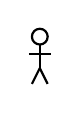
\begin{tikzpicture}[scale=0.4]
      \draw[fill=white, line width=0.8pt] (0,1) circle (0.25);
      \draw[line width=0.8pt] (0,0.75) -- (0,0);
      \draw[line width=0.8pt] (-0.35,0.45) -- (0.35,0.45);
      \draw[line width=0.8pt] (0,0) -- (-0.25,-0.5);
      \draw[line width=0.8pt] (0,0) -- (0.25,-0.5);
    \end{tikzpicture}\\
    \small Administrateur /\\Crawler
  };

  % Frontière du système
  \begin{scope}[on background layer]
    \node[group-box, fit=(titleNode) (uc1) (uc2) (uc3) (uc4) (uc5) (uc6), inner xsep=0.4cm, inner ysep=0.4cm] (system-boundary) {};
  \end{scope}

  % Connecteurs de l'Utilisateur Final
  \draw[flow-arrow] (user.east) -- (uc1.west);
  \draw[flow-arrow] (user.east) -- (uc2.west);
  \draw[flow-arrow] (user.east) -- (uc3.west);
  \draw[flow-arrow] (user.east) -- (uc4.west);

  % Connecteurs de l'Administrateur
  \draw[flow-arrow-gold] (admin.west) -- (uc5.east);
  \draw[flow-arrow-gold] (admin.west) -- (uc6.east);
\end{tikzpicture}
\caption{Diagramme de cas d'utilisation de la plateforme}
\label{fig:use_case}
\end{figure}